\chapter{Reference Nets}
\label{ch:reference}

First, we are going to take a look at Petri nets with Java as an
inscription language. Then we look at synchronous channels
and net references, two extensions that greatly add
to the expressiveness of Petri nets as described in~\cite{Kummer98}
and \cite{Kummer99}.
Finally, we are going to see how nets and Java can
seamlessly interact with each other.
Reference nets and their theoretical foundation as a whole are
defined in \cite{Kummer2002:diss} (in German).

\section{Net Elements}

Reference nets consist of \emph{places}, \emph{transitions}, and
\emph{arcs}.

There are many types of arcs. Firstly, ordinary
\emph{input} or \emph{output arcs} that come with a single arrow head.
These behave just like in ordinary Petri nets, removing or depositing
tokens at a place. Secondly, there are \emph{reserve arcs}, which are simply
a shorthand notation for one input and one output arc. Effectively, these
arcs reserve a token during the firing of a transition. Thirdly, there
are \emph{test arcs}, which have no arrowheads at all. A single token may be
accessed, i.e.\ tested, by several test arcs at once. This is
important, because an extended period of time might be needed before
a transition can complete its firing. For a more detailed treatment
of test arcs see~\cite{CDH93}.

Besides these basic arc types, there are arc types that add
greatly to the expressiveness of nets, but are not as easy
to understand. We postpone the description of these arcs until
Section~\ref{sec:additionalArcs}.

Each place or transition may be assigned a \emph{name}. Currently,
this name is used only for the output of trace messages.
By default, names are displayed in bold type.

\singlenet{elements}

In Fig.~\ref{fig:elements} you can see a net that uses all
net elements that were mentioned so far. You can find it in
the directory \texttt{samples/simple} of the Renew distribution.
A single place~\texttt{p}
is surrounded by six transitions. Initially, the place is unmarked.
Assume that transition~\texttt{a} fires, which is always
possible, because all its arcs are output arcs. Now one token
is placed in~\texttt{p}, and all transitions except~\texttt{c} are
activated. Transition~\texttt{c} is still disabled, because it reserves
\emph{two} tokens from~\texttt{p} while it fires. In contrast to this,
transition~\texttt{e} may fire, because it is allowed to test
a single token twice.
If~\texttt{a} fires again, transition~\texttt{c} becomes activated,
too, because a second token is now available. A firing of
the transitions \texttt{b}, \texttt{c}, \texttt{e}, and \texttt{f}
does not change the current marking. However, transition~\texttt{d}
will remove one token from \texttt{p} during each firing.

Every net element can carry semantic inscriptions.
Places can have an optional \emph{place type} and an arbitrary number of
\emph{initialization expressions}. The initialization expressions are
evaluated and the resulting values serve as initial markings
of the places. In an expression, \texttt{[]} denotes a simple black token.
By default, a place is initially unmarked.

Arcs can have an optional \emph{arc inscription}. When a transition
fires, its arc expressions are evaluated and tokens are moved
according to the result.

Transitions can be equipped with a variety of inscriptions.
\emph{Expression inscriptions} are ordinary expression that are evaluated
while the net simulator searches for a binding of the transition.
The result of this evaluation is discarded, but in such expressions
you can use the equality operator~\texttt{=} to influence the binding
of variables that are used elsewhere.

\emph{Guard inscriptions} are expressions that are prefixed with the reserved
word \texttt{guard}. A transition may only fire if all of its
guard inscriptions evaluate to \texttt{true}.

\singlenet{colored}

With these additions we cover the basic colored
Petri net formalism. In Fig.~\ref{fig:colored}, which is
also provided in the directory \texttt{samples/simple}, we find a net
that uses the basic place and arc inscriptions. At the left,
we have a place that is typed \texttt{int}, which means that it
can only take integers as tokens. In this case, it has an initial
marking of one integer \texttt{42} token. The other places
are untyped and initially unmarked. The leftmost transition
will take \texttt{42} out of the place and deposit one \texttt{4}
and one \texttt{2} into the respective places. The upper middle
transition takes some \texttt{x}, which happens to be \texttt{4}
in this case, out of its input places and copies it into its
two output places. The lower middle transition is similar,
but here the equality of input and output arc variables
is established by the transition inscription \texttt{x=xx}.
The rightmost transition has a guard that ensures that
$\texttt{x}\neq \texttt{y}$, written \texttt{guard x!=y}.
Therefore it can only take a \texttt{2} out of the upper place
and a \texttt{4} out of the lower place or vice versa.

\emph{Action inscriptions} are expression inscriptions preceded with the
keyword \texttt{action}. Contrary to expression inscriptions,
action inscriptions are guaranteed to be evaluated exactly once during
the firing of a transition. Action inscriptions cannot be used
to calculate the bindings of variables that are used on input arcs,
because input arc expressions must be fully evaluated before a transition
can fire. However, action inscriptions can help to calculate output
tokens and they are required for expressions with side effects.

Then there are \emph{creation inscriptions} that deal with the creation
of net instances (see Section~\ref{sec:netinst}) and
\emph{synchronous channels}
(see Section~\ref{sec:channels}). But first we will look closer
at the expression syntax, which is very similar to a subset of Java.
In fact, we have to look carefully to spot the differences.


\section{I do not Want to Learn Java}

Even if you do not want to learn Java, Renew might be a useful
tool for you, although it looses some of its expressiveness.
In many cases it is enough to learn how to write numbers,
strings, variables, and the simplest operators.

Reference nets provide extensions that go well beyond
simple high-level Petri nets with Java inscriptions.
After you have read the next sections, you can use these
extensions to generate complex models without the need to
incorporate Java code.

But remember that there are always subproblems that are
easier to express in a programming language rather than
Petri nets. Reference nets work together seamlessly with Java programs
and gain a lot from utilizing the Java libraries.
So once you \emph{do} learn Java, you can choose the
appropriate modeling method for each task at hand.


\begin{table}
  \begin{center}
    \begin{tabular}{ll}
      \texttt{boolean} & boolean values (\texttt{true}, \texttt{false})\\
      \texttt{byte} & 8-bit signed integers \\
      \texttt{short} & 16-bit signed integers \\
      \texttt{int} & 32-bit signed integers \\
      \texttt{long} & 64-bit signed integers \\
      \texttt{char} & 16-bit unsigned Unicode characters \\
      \texttt{float} & 32-bit IEEE floating point numbers \\
      \texttt{double} & 64-bit IEEE floating point numbers \\
    \end{tabular}
  \end{center}
  \caption{The primitive data types of Java}
  \label{tab:primtypes}
\end{table}


\section{A Thimble of Java}

If you are already familiar with Java, you will want to skip
to Section~\ref{sec:inscrlang} where we discuss the differences
between Java and the inscription language used in reference nets.
Here we give a most rudimentary introduction to Java.

Java is an \emph{object-oriented} programming language, but
not everything is an object in Java. There are eight
non-object data types in Java which are listed in
Table~\ref{tab:primtypes}. The types \texttt{byte},
\texttt{short}, \texttt{char}, \texttt{int}, and \texttt{long}
are called integral types here. Together with \texttt{float}
and \texttt{double} they form the number types.

In Figure~\ref{fig:primtyp} you can see two type hierarchies.
On the left the ordinary Java subtype relation is depicted.
You can see that \texttt{long} is a subtype of \texttt{float}
although some loss of precision might occur during the conversion.
Nevertheless, Java will silently insert this conversion whenever
it is required in a program.

\begin{figure}[tbp]
  \centerline{%
    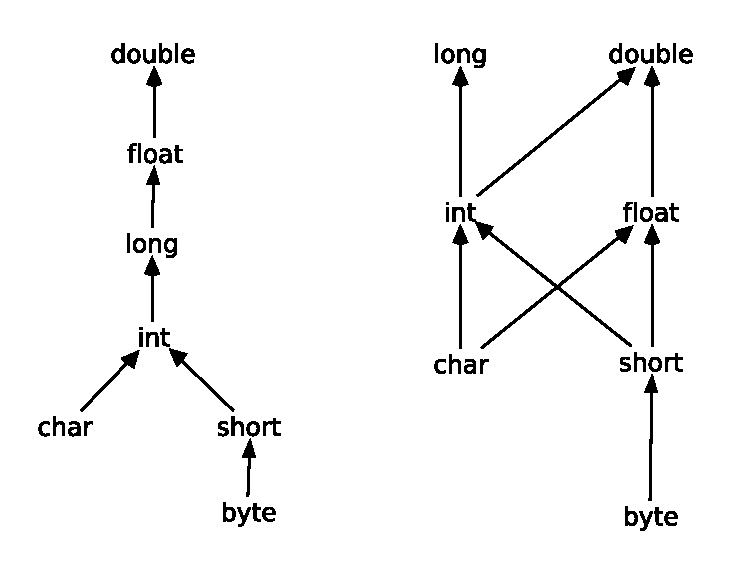
\includegraphics[scale=\netscale]{primtyp.eps}%
    }
  \caption{\label{fig:primtyp}The Java type hierarchy and the hierarchy
    of lossless conversions}
\end{figure}%

Although this is helpful for Java programs, it poses
several problems in the context of Petri nets, where the
direction of information transfer is not always immediately
obvious. Hence such conversions are not done by the simulator.
Instead we introduced the relation of lossless conversions,
which you can find on the right hand side of
Figure~\ref{fig:primtyp}. This relation governs the
type constraints between places and their neighboring arcs.

All other types except primitive types
are \emph{reference types}, i.e., references to some
object. Every object belongs to a \emph{class}. When a class is declared,
it may receive an arbitrary number of field declarations and
method declarations. \emph{Fields} are variables that exist once per
object or once per class. The binding of the fields of an object
captures the state of that object.
\emph{Methods} describe the possible actions of an object.
Each method has a name, a list of parameters, and a body, i.e.~a
sequence of statements that are executed if the method is invoked.

%Hence methods are related to transitions in a Petri net,
%although they cannot occur spontaneously. Fields are
%similar to places in a Petri net, but they hold exactly
%one value at each time.

Method declarations and field declarations are nested in the
declaration of the class to which they belong. It is possible to use
the predefined classes without writing new ones, when working with
Renew. We are going to see later how nets themselves can be regarded as
classes. For a detailed
discussion of the Java type system and the Java system libraries
we refer the reader to the literature.

Now we are going to look at the syntax of Java expressions. We only
deal with the subset of Java that is relevant to reference nets.

\emph{Variables} are represented by identifiers. Identifiers are
alphanumeric strings starting with
a non-numeral character. E.g., \texttt{renew}, \texttt{WRZLGRMF},
\texttt{go4it}, and \texttt{aLongVariableName} are all
valid variable names. By convention, variable names should start
with a lower case character. The declaration of a variable
is denoted by prefixing the variable name with the type name,
e.g.\ \texttt{int i}. Variables were already silently assumed in
Fig.~\ref{fig:colored}.

The Java language provides \emph{literals} for integers (\texttt{123}),
long integers (\texttt{123L}), floats (\texttt{12.3F}),
and doubles (\texttt{12.3}). Furthermore, there are the boolean
literals \texttt{true} and \texttt{false}, string literals
(\texttt{"string"}), and character literals (\texttt{'c'}).
Java uses 16-bit Unicode characters and strings. There
are no literals for the primitive types byte and short.

There is also one literal of reference type named \texttt{null}.
Every variable of a reference type may take \texttt{null} as a value.
\texttt{null} equals only itself and no other reference.
Trying to invoke a method of the \texttt{null} reference will
fail with a runtime exception.

A sizable set of \emph{operators} is provided in Java.
Here we are going to discuss those operators that are still
present in reference nets.
The binary operators are listed in Table~\ref{tab:operators},
where we also note their interpretation and the operand types
to which each operator is applicable.

\begin{table}
  \begin{center}
    \begin{tabular}{lll}
      \texttt{*} & multiply & number \\
      \texttt{/} & divide & number \\
      \texttt{\%} & modulo & number \\\hline
      \texttt{+} & plus & number, \texttt{String} \\
      \texttt{-} & minus & number \\\hline
      \texttt{<<} & shift left & integral \\
      \texttt{>>} & shift right & integral \\
      \texttt{>>>} & signed shift right & integral \\\hline
      \texttt{<} & less than & number \\
      \texttt{>} & greater than & number \\
      \texttt{<=} & less than or equal & number \\
      \texttt{>=} & greater than or equal & number \\\hline
      \texttt{==} & equal & primitive, reference \\
      \texttt{!=} & unequal & primitive, reference \\\hline
      \texttt{\&} & and & primitive \\\hline
      \texttt{\^{}} & exclusive or & primitive \\\hline
      \texttt{|} & or & primitive \\
    \end{tabular}
  \end{center}
  \caption{Java binary operators,
    rules separate operators of equal precedence}
  \label{tab:operators}
\end{table}

Most of the operators are defined for primitive types only,
but you can also check if two references are identical with
\texttt{==} and \texttt{!=}.

\bug{Never use \texttt{==} or \texttt{!=}
to compare the equality of strings, like in
\texttt{s1==s2}. Always use the Java-method \texttt{equals(...)}
as in \texttt{s1.equals(s2)} or you will get strange results.
This is a peculiarity
that annoys many Java beginners, but we are not in a position
to change this behavior.}

The operator \texttt{+}
is also used to concatenate strings. If only one operand
of~\texttt{+} is a string, the other operand is first
converted to a string and the two strings are concatenated
afterward, e.g.\ \texttt{"7x8="+42} results in the string
\texttt{"7x8=42"}.

If multiple operators are present, they are grouped according to
their \emph{precedence}. \texttt{*}, \texttt{/}, and \texttt{\%}
have the highest precedence, \texttt{|} has the lowest precedence.
The expression \texttt{a+b\%c*d|e} is equivalent to the
fully parenthesized expression \texttt{(a+((b\%c)*d))|e}.
The order of precedence for each operator
can be found in Tab.~\ref{tab:operators}.
If in doubt, make the parentheses explicit.

An operand of a small type
(\texttt{byte}, \texttt{short}, or \texttt{char}) is automatically
converted to \texttt{int} before any operator is applied. If
you need the result as a small type, you have to make an
explicit \emph{cast}. E.g., \texttt{(byte)b1+b2} adds the two bytes
\texttt{b1} and \texttt{b2} and truncates the result to
8 bits. You might also want to reduce the precision of a
floating point number by saying \texttt{(float)d1} where
\texttt{d1} is a \texttt{double} variable. The opposite case where
precision is added, e.g.\ \texttt{(long)b1}, is helpful, too,
but usually this kind of conversion is added automatically
in the places where it is needed.

Casts between reference types are also possible, but here no
conversion takes place. Instead, it is checked that the operand
is indeed of the given reference type, either at compile time
or at run time, if required. E.g., if a variable \texttt{o}
of type \texttt{Object} is declared, we can say \texttt{(String)o}
to ensure that \texttt{o} does indeed hold an object of type
\texttt{String}.

There are a few unary operators, too. They are listed in
Table~\ref{tab:unary}. Unary operators and casts have a higher operator
precedence than any binary operator.

\begin{table}
  \begin{center}
    \begin{tabular}{lll}
      \texttt{-} & negate & number \\
      \texttt{\~{}} & bit complement & integral \\
      \texttt{!} & not & boolean \\
    \end{tabular}
  \end{center}
  \caption{Java unary operators}
  \label{tab:unary}
\end{table}

A last operator that must be mentioned
is \texttt{instanceof}. Its left operand is an expression
as usual, but its right operand must be the name of a class or interface.
It evaluates to true, if the result of the expression is
a reference to an object of the given class or one of its subclasses
or of a class that implements the given interface.

With an object reference you can also inspect fields and invoke
methods. E.g., if there is an object \texttt{o} with a field \texttt{f},
you can access the field by writing \texttt{o.f} inside a Java expression.
The result will be the current value of that field.

For an object \texttt{o}, a call of the method \texttt{m} with the parameters
\texttt{1} and \texttt{x} would look like \texttt{o.m(1,x)}.
This has the result of binding the formal variables to the parameter values
and executing the body statements of the method. Unless the method is
of the return type \texttt{void}, a return value will be calculated and
returned.

Due to \emph{overloading},
there might be more than one method of a given name within some class.
In that case, the method that matches the parameter types
most closely is invoked.

In order to create a new instance of a class, you can use the
\texttt{new} operator. E.g., the expression
\texttt{new java.lang.StringBuffer()}
will create a new object that belongs to the class \texttt{java.lang.StringBuffer}
and invoke its \emph{constructor}. A constructor can be seen as a special
method that initializes a new object. The \texttt{new} operator
can take arguments inside the parentheses. The arguments are then passed
to the constructor just as in an ordinary method call.


\section{The Inscription Language}
\label{sec:inscrlang}

Because we are dealing with a colored Petri net formalism,
the net simulator must determine which kind of token is moved for
each arc.

The possible kinds of tokens are Java values or references.
By default, an arc will transport a black token,
denoted by \texttt{[]}. But if you add an
\emph{arc inscription} to an arc, that inscription will be evaluated
and the result will determine which kind of token is moved.

\subsection{Expressions and Variables}

Arc inscriptions are simply Java expressions, but there are a
few differences.
The first difference concerns the operators that are used in
expressions. In Java the binary operators \verb:&&: (logical and)
and \verb:||: (logical or) are short-circuit operators. I.e., if the
result of the left operand determines the result of the operator,
the right operand is not even evaluated. This would imply
an order of execution, which we tried to avoid in our net formalism.
Hence, the two operators are not implemented.
The same holds for the ternary selection operator \verb|?:|.
An additional benefit of its exclusion from the language is
that this frees up the colon for other
syntactic constructs. Possibly, these three operators might
still occur in later releases of Renew.

In Java
variables receive their value by \emph{assignment}. After a second
assignment, the value from the first assignment is lost.
This flavor of variables is not well-suited for high-level
Petri nets. Instead variables are supposed to be bound to one
single value during the firing of a transition and that value
must not change.
However, during the next firing of the same
transition, the variables may be bound to completely different values.
This is quite similar to the way variables are used in logical
programming, e.g.~in Prolog.

\singlenet{gcd}

In Fig.~\ref{fig:gcd} we show an example net that uses
expressions as arc inscriptions and also as guard inscriptions.
The example is provided in the directory \texttt{samples/simple}.
Some numbers are put into a place and the net will compute
the greatest common divisor of all these numbers and terminate
with no more enabled transitions. The upper central transition is the
most interesting. It removes two tokens from the pool of numbers,
but a guard makes sure that the two numbers are greater than
zero and correctly ordered. The transition outputs the smaller number
and the remainder (denoted by the operator \texttt{\%})
of the division of the greater number by the smaller number.
The lower central transition simply puts the new numbers
back into the pool and the left transition discards zeroes.

Note how a single variable can be bound to different values
at different times. Note that the simulator will automatically search
for possible bindings of the variables.


\subsection{Types}
\label{subsec:types}

For reference nets, types play two roles. A type may be
an inscription of a place. This means that the place can hold only
values of that type. The net simulator can statically detect
many situations where type errors might occur, i.e., when transitions
try to deposit tokens of the wrong type into a place.
Furthermore, variables may be typed. This means that the variable
can only be bound to values of that type.

In Java every variable needs to be declared. There are of course
many good reasons to demand this, but there are times when
it is valuable to write programs without having to worry
about a type declaration. One of these cases are throw-away
prototypes, which are supposed to be developed very quickly.
Petri nets are generally usable for prototyping, so we wanted
to be able to write nets without having to declare variables.

But for stable code that will be used in a production application
types are a must. Therefore reference nets provide the option
to create a \emph{declaration node}. In the declaration node,
an arbitrary number of Java import statements and Java
variable declarations are allowed. If a declaration node is present,
then \emph{all} variables must be declared. This means that
you have the choice between complete liberty (no variables
can be declared) and complete security (all variables must
be declared).

Note that an undeclared variable does not have a type. Therefore,
the type of an expression can only be determined at runtime,
if it contains undeclared variables. Worse, if a method is
overloaded, the choice of the actual method must be
delayed until runtime when all operator types are known.
This is contrary to ordinary Java, where overloaded methods
are disambiguated at compile time.

\singlenet{gcdtyped}

Fig.~\ref{fig:gcdtyped} shows a typed variation of the greatest
common divisor algorithm. First, you can see the type inscriptions
of the places that are all \texttt{int} in this case. Second,
you will notice the declaration node where the two variables
are declared. As in Java, declarations consist of the type
followed by the name of the variable.

Places can be typed, too. This allows the
simulator to catch some difficult situations before the
actual simulation. For input arcs, the type of the arc inscription
should be comparable to the type of the place, i.e.\ either
a subtype or a supertype. Otherwise
it is probable that the expression yields a value that cannot be
a token in the place. Note that for this type check we have to use the
lossless conversion rules as depicted in Figure~\ref{fig:primtyp}

For output arcs we require that the type
of the arc expression is narrower than the type of the place, so that
the place can always take the resulting token. This is
important, because the values of the output expressions might
only be determined during the firing of the transition when it is
too late to declare the transition disabled. For input arcs we can
simply ignore any binding that would result in a token
of a bad type.

As a special case it is required that an output arc expression
for a typed place must be typed. In practice this means that you have
to declare your variables as soon as you assign types to places.
On the other hand, you can type the variables without having to type
the places.

Sometimes it is required to convert an expression of one type to an
expression of a different type. Reference nets support Java's
concept of \emph{casts}. A cast is indicated by prefixing
an expression with the desired type enclosed in parentheses.
E.g., \texttt{(Object)"string"} would be an expression
of type \texttt{Object}, even though it will always
result in \texttt{"string"}, which is of type \texttt{String}.

On the other hand, if you know that a variable \texttt{o} of type
\texttt{Object} will always hold a string, you can say
\texttt{(String)o} to inform the type system of this
fact. For primitive types, a conversion
takes place, e.g., \texttt{(byte)257} converts the 32-bit
integer \texttt{257} into the 8-bit integer \texttt{1} by
truncating the most-significant bits.

In Fig.~\ref{fig:gcdtyped} we also illustrated that you can
make multiple inscriptions to a single transition, as we have
two guards for a single transition.

If multiple transition inscriptions are
given in a single graphical figure as in this case,
the inscriptions have to be separated by semicolons.
They may also optionally be terminated with a semicolon.


\subsection{The Equality Operator}
\label{subsec:equality}

If we look at the new semantics of variables, we might wonder
what the meaning of the operator~\texttt{=} is.
It cannot be an assignment, because variables are immutable.
Instead, it is merely a specification of equality. You will usually
want equality specifications to occur inside special inscriptions
that are attached to transitions. E.g., you can say
\texttt{x=2} to bind the variable \texttt{x} to 2 or you could
use \texttt{x=y*z+42} for a more interesting computation.
If you specify both \texttt{x=2} and \texttt{x=3} for a single
transition, that transition will not be able to fire, because
\texttt{x} cannot be bound in a way that matches both specifications.

Keep in mind that \texttt{=} is based on equality in the
sense of the \texttt{equals(Object)} method and not in the sense of
the operator \texttt{==}. This might confuse experienced Java
programmers, but it is the only possibility to avoid certain other
anomalies.

\singlenet{equality}

In the net from Fig.~\ref{fig:equality} you can see two transitions
that perform equivalent actions, as you can see when you
load the nets from \texttt{samples/simple} and simulate them. The
transition on the right uses a variable \texttt{z} to hold the value of the
computation \texttt{x+y}. At the left we see an example where an expression
occurs on an input arc. Such expressions are properly evaluated
and the simulator checks whether the resulting token is available.

But expressions on input arcs have to be used with care.
Just because the simulator knows that \texttt{x+y} equals \texttt{24}
and \texttt{x} equals \texttt{22}, it cannot conclude that
\texttt{y} is \texttt{2}. Such computations would have been
possible in some cases, but not in others. Due to consistency
we decided on the general rule that expressions are not evaluated
backward. The only exception are type casts, which we met earlier on.
A type cast that may be performed without losing information,
e.g.\ \texttt{(long)i} for an integer \texttt{i},
can be calculated backward.
If due to an equality specification the result of such a cast
is known, it is propagated backward to the casted expression,
possibly after some conversion.

If a backward computation is desired in the other cases,
it has to be made explicit. In our example, we could
complement the equation \texttt{z=x+y} by \texttt{x=z-y}
and \texttt{y=z-x}. Now the simulator can determine \texttt{y} from
\texttt{x}~and~\texttt{z}. This is allowed, exactly because
\texttt{=} does not mean an assignment but an equality specification.
If a bound variable is calculated again by a redundant
equation, this does not pose a
problem as long as the two bindings are equal.

If \texttt{=} does not assign,
what do the modifying operators \texttt{+=},
\texttt{*=}, and so on mean in reference nets? Simple answer: They
make no sense and were therefore excluded from the language.
Similarly, the operators \texttt{++} and \texttt{--} do not
appear.

\subsection{Method Invocations}

Reference nets also support method invocations.
E.g., \texttt{x.meth("a")} invokes the method \texttt{meth} of the
object referenced by \texttt{x} with the parameter string \texttt{"a"}.
All Java methods can be used in reference nets, but there are
some critical points.

First of all, methods can be evaluated more than once. Worse,
a method might be invoked even though the transition does not fire.
This is done, because the result of a method invocation might
be needed to determine whether a transition is enabled at all.
Therefore it is best, if the invoked methods do not produce
any side effects.
If side effects are required, then they should be
invoked in action inscriptions only.

\singlenet{frame}

Fig.~\ref{fig:frame} shows some example method calls that
are invoked by net inscriptions.
The net is saved in the directory \texttt{samples/simple}.
The declaration node contains an \emph{import statement}
that instructs the simulator to search the package \texttt{java.awt}
for classes whose names appear in the net. The variables
\texttt{f} and \texttt{b} are then declared as a \texttt{Frame}
and a \texttt{Button}. These two classes are
in the package \texttt{java.awt}, so we could have written
\texttt{java.awt.Frame} and \texttt{java.awt.Button} instead.
The procedure that has been implemented here is simple.
A window and a button are created, the window is resized
and the button is added to the window. Now we can show the window,
let the user click it some times, and remove it from the screen
again.

It is possible to give multiple actions in a single transition
inscription in a semicolon separated list, e.g.,
\texttt{action y=o.m(x); action x=o.m();} would be allowed.
Note that the order of execution need not match the textual
order. In the previous example, \texttt{action x=o.m()} would
have to be executed first, because it is required to determine
the binding for \texttt{x}. In the same sense, the \texttt{action}
keyword only applies to a single expression, not to all following
expressions. E.g., \texttt{action y=o.m(x); x=o.m();} would
mean that \texttt{x=o.m()} is evaluated early during the
search for a binding, because it is not an action.

\section{Tuples, Lists, and Unification}
\label{sec:tuplist}

The inscription language of reference nets has been extended
to include \emph{tuples}. A tuple is denoted by a comma-separated list
of expressions that is enclosed in square brackets. E.g.,
\texttt{[1,"abc",1.0]} denotes a 3-tuple which has as its
components the integer 1, the string \texttt{"abc"}, and
the double precision float 1.0. Tuples are useful for storing
a whole group of related values inside a single token
and hence in a single place.

In ordinary Java, there are no tuples. If we want to store a
group of values, we can simply create a group of variables,
each of which holds one value. But with Petri nets we want to
store arbitrarily many tokens in a place, making this solution
useless in many cases.

It would of course be possible to
create a Java class with an appropriate set of fields
to wrap a group of values, but this would result
in an excessive amount of trivial functionless classes.
(By the way, this is what has to be done in Java in some cases, too.)

Tuples are weakly typed. They are of type \texttt{de.renew.unify.Tuple},
but their components are untyped. It is not even specified
whether a component of a tuple holds a primitive or
a reference type.

This does not matter much, because the only operation on tuples
(or rather the only operation that should be used) is
\emph{unification}. You can unify tuples through an equality
specification. E.g., \texttt{[x,y,z]=t} means that
\texttt{t} must be a 3-tuple. Furthermore, \texttt{x} will be
equal to the first component of \texttt{t}, \texttt{y} to the second,
and \texttt{z} to the third.

We already know that the black token is denoted by \texttt{[]}.
Therefore a black token is simply a tuple without components
(a zero-tuple).

\singlenet{socks}

In Fig.~\ref{fig:socks} we can see the sock algorithm of the typical
theoretical computer scientist. The scientist will reach into the
drawer to fetch two socks. It does not matter if the
socks are left socks or right socks (they are topologically equivalent)
as long as they are of the same color.
In the net, which can be found in the
directory \texttt{samples/tuple}, this is achieved by using the
variable \texttt{col} in both arc inscriptions that will remove
tokens from the \texttt{drawer} place.

Tuples may be nested. \texttt{[[1,2],[3,4,5]]} would be a 2-tuple
that has a 2-tuple as its first component and a 3-tuple
as its second component. This might be useful if the components
are hierarchically structured.

It is a common task to use tuples to simulate a database,
so that the number of tuples in a place can be
considerable. Often one component of an input arc tuple can be determined
without accessing the place. In this case, Renew
accesses only those tokens that match the known component. Because few
tokens need to be checked, the simulation can proceed quickly.
If \emph{two} components of the input arc tuple
are known, the simulation engine will use that component as
a key that results in fewer matches.

In functional programming
nested pairs are used as a representation of lists.
This could be simulated by nested tuples, but it would
result in nets that are hard to read. Hence we added
explicit list support to the language.
Lists are delimited by curly braces, e.g., \verb|{1,2,3,4}|
would be a four element list. Lists, like tuples, support pattern
matching. Using \verb|{1,2,3,4}={u,v,w,x}| as a transition
inscription, we would get \texttt{u=1}, \texttt{v=2}, and so on.

\singlenet{reverse}

In order to handle lists of unknown length, a tail expression
may be added to the list. The tail expression is separated
from the ordinary list elements by a colon. The tail expression
matches an arbitrary list of elements.
By requiring \verb|{1,2,3,4}={u,v:w}| we get
\texttt{u=1}, \texttt{v=2}, and \verb|w={3,4}|. The tail
consists of all elements that are not explicitly represented.
The tail may be empty as in \verb|{1,2,3,4}={u,v,w,x:y}|
where \verb|y={}|. Note that the empty tuple \texttt{[]}
and the empty list \verb|{}| are not equal.

In Fig.~\ref{fig:reverse} you can see an example net, which reverses
a list by successively splitting off the head of the original list
and appending it to a result list. The remainder of the
original list and the result list are jointly contained
in a tuple. Once the original list is fully consumed, the result
list is extracted.


\section{Net Instances and Net References}
\label{sec:netinst}

When a simulation run of a net is started, the simulator creates
a \emph{net instance} of the net that is simulated.
A net that is drawn in the editor
is a static structure. However, an instance of the net has a
marking that can change over time. Whenever a simulation is started,
a new instance is created.

Most net formalisms stop here. They create one instance of a net
and simulate it. Renew allows you to create many instances
of a single net. Each instance comes with its own marking
and can fire independently of other instances.

Every net has a \emph{name}. The name is derived from the file
where it is saved by removing the directory name and
the suffix. E.g., a net saved in \texttt{/users/foo/bar/baz.rnw}
would have \texttt{baz} as its name.

New net instances are created by transitions that carry
\emph{creation inscriptions}, which consist of a variable name,
a colon~(\texttt{:}), the reserved word \texttt{new}, and
the name of the net. E.g., \texttt{x:new baz} makes sure that
\texttt{x} is bound to a fresh instance of the net \texttt{baz}.

In Figs.\ \ref{fig:creator}~and~\ref{fig:othernet} you can see
a simple example. These nets are available in the \texttt{samples/creation}
directory.

\doublenet{creator}{othernet}

When you start a simulation of \texttt{creator}, the top transition
can fire and creates two new net instances of \texttt{othernet}.
References to the two nets are deposited in the middle places.
Now \emph{three} transition instances are activated, namely
the two transitions in the two instances of \texttt{othernet} and
the bottom transition of \texttt{creator}. The guard is satisfied, because
two different creation inscriptions are guaranteed to create different
net instances. You never create the same instance twice.

Now the order of execution is undefined. It might be possible
that the bottom transition of \texttt{creator} fires first.
Even in that case, the two transitions instances of \texttt{othernet}
remain activated. A net does not disappear simply because it is no
longer referenced.

On the other hand, if a net instance is no longer referenced and none
of its transition instances can possibly become enabled, then it
is subject to garbage collection. Its presence has become undetectable
and hence we might remove it without further ado.

In Java the reserved word \texttt{this} denotes the object whose method
is currently executed. In reference nets \texttt{this} denotes
the net instance in which a transition fires.

We are often going to treat net instances like objects of an object-oriented
programming language. They are instances of a net, just like objects
are instances of a class. They have an identity that can be checked
with \texttt{==} and \texttt{!=} just like objects. They have a state
that can change over time and here places seem to correspond to
attributes. Net instances also encapsulate data. They can be referenced
from other net instances. The only missing component for full objects
are methods. In the next section we will learn about a communication
concept that can be substituted for method calls sometimes.
In Sec.~\ref{sec:netcall} we will finally see how nets can be equipped with
methods.


\section{Synchronous Channels}
\label{sec:channels}

Currently, the idea of net instances might not seem interesting, because
there is no mechanism by which nets can influence each other.
Hence, although net instances encapsulate data, they encapsulate it
so well that it cannot be accessed at all.

\singlenet{synchro}

In this section we will establish a means of communication for net
instances. There are two fundamentally different ways of communication.
First, we have message passing where a sender creates a message that can be
read by a receiver later on. The sender can always send the message
regardless of the state of the receiver. The receiver may or may not
be able to process the message.
Second, we have synchronous communication where sender and receiver
have to agree on participating in an communication at some point of
time.

In Petri net formalisms, the former kind of communication is usually
captured by so-called fusion places.
Reference nets, though, implement the latter kind of communication
in the form of \emph{synchronous channels}.
This allows more expressive models compared to message passing,
because it hides much of the inherent complexity
of synchronization from the developer.
Furthermore, message passing can
always be simulated using synchronous communication.

Synchronous channels were first considered for colored Petri nets
by Christensen and Damgaard Hansen in~\cite{CDH92}. They synchronize
two transitions which both fire atomically at the same time.
Both transitions must agree on the name of the channel and on
a set of parameters, before they can engage in the synchronization.

Here we generalize this concept by allowing transitions
in different net instances to synchronize. In association with classical
object-oriented languages we require that the initiator
of a synchronization knows the other net instance.

The initiating transition must have a special inscription, the
so-called \emph{downlink}. A downlink makes a request at
a designated subordinate net. A downlink consists of an expression
that must evaluate to a net reference, a colon~(\texttt{:}),
the name of the channel, an opening parenthesis, an optional
comma-separated list of arguments, and a closing parenthesis.
E.g., \texttt{net:ch(1,2,3)} tries to synchronize with another transition
in the net denoted by the variable \texttt{net},
the channel has the name \texttt{ch} and is passed the parameters \texttt{1},
\texttt{2}, and \texttt{3}.

On the other side, the transition must be inscribed with a
so-called \emph{uplink}. An uplink serves requests for everyone.
A transition that is called through an uplink need not know the
identity of the initiator, just like an activated method of an object
does not necessarily know of its caller.
Therefore the expression that designates the other net instance
is missing for uplinks. An example uplink inscription
would look like \texttt{:ch(x,y,z)}, which means that
the channel name is \texttt{ch} and that the three channel
parameters must match the binding of the variables \texttt{x},
\texttt{y}, and \texttt{z}.

The uplinks and downlinks of a transition may be
given as individual transition inscriptions or in a single
semicolon separated list in one inscription. The list might
even include action inscriptions and creation inscriptions
simultaneously with the channel invocations.

Let us first look at the special case where two net instances
within the same net synchronize. This is done by providing
the keyword \texttt{this} as the target of the downlink.
In Fig.~\ref{fig:synchro} you can see an example net with local
channels, which is provided in the directory \texttt{samples/channel}
like all other nets of this section.
The input place of the left transition
is marked and the transition's downlink specification can be
met by synchronizing with the right transition. Both transitions
fire synchronously, such that one token is removed from
the left place and one token is added to the right place
in a single step.
Now no more transitions are enabled. The left transition
lacks a token on its input place, the right
transition has an uplink that is not invoked by another transition.

Generally, transitions with an uplink cannot fire without being
requested explicitly by another transition with a matching downlink.
We will sometimes call a transition without an uplink
a \emph{spontaneous} transition. But even a spontaneous transition
must find an appropriate synchronization partner if it has a downlink.

It is allowed that a transition has multiple downlinks. It is also
allowed that a transition has both an uplink and downlinks. This is
exemplified in Fig.~\ref{fig:multi}. Again the transition on the left
initiates the synchronization. The required channel is offered by the
middle transition which does nothing except linking to the channel
\texttt{bar} twice. This is allowed, a transition may fire multiple
times in one synchronous step, although it might be confusing and
should be avoided when possible.

In general, multiple levels of synchronization are suspect from a
methodical point of view, because they tend to be difficult to understand.
Petri nets excel at displaying control flow and it seems that
synchronous channels should not be used to encapsulate complex
control flows or even loops. It is best to use channels where they
show their greatest potential, namely synchronization,
communication, and atomic modifications.

\singlenet{multi}

Channels can also take a list of parameters. Although there is a
direction of invocation, this direction need not coincide with the
direction of information transfer. Indeed it is possible that a
single synchronization transfers information in both directions.
Fig.~\ref{fig:param} shows a possible application where the
left transition consults a lookup table that is managed
by the right net instance. The parameter lists \texttt{(x,y)} and
\texttt{(a,b)} match if \texttt{x=a} and \texttt{y=b}. After binding
\texttt{x} from the left place the variable \texttt{a}
is determined and only one token of the right place matches
the tuple of the arc inscription. This allows to bind \texttt{b}
and hence \texttt{y}.

\singlenet{param}

In the previous examples we only encountered local synchronizations
within one net, but Figs.\ \ref{fig:santa}~and~\ref{fig:bag}
show two separate nets that can communicate. The net represents
the basic schedule of Santa Claus on the night before Christmas.
He wakes up, takes a new bag from the shelf and fills it with
presents. Later on he can simply reach into his bag
and get something that he can put into the children's boots, maybe
some candy or a brand new game.

\doublenet{santa}{bag}

It is possible to create synchronization loops where the invocation of a
channel results in the invocation of the same channel.
This should be avoided, because it might throw the simulator into
an infinite loop. A different search strategy could have avoided
this problem, but it would have incurred a significant performance
cost.

We mentioned that message passing can be simulated by synchronous channels.
The canonical way would be to create a transition with
a single-parameter uplink
and a single output arc in the receiving net, which can then
put the argument of its uplink into its output place. Because this
transition is always enabled, messages can always be sent and
the state of the receiver does not influence the sender in any way.
After the message has been put into the place, it can be processed
in an arbitrary way.

Using the special inscription \texttt{x:new net()} you can
indicate that you want to create a new net with name \texttt{net},
assign it to the variable \texttt{x} \emph{and} perform a
synchronization with the uplink \texttt{:new()} in the newly
created net in one step. Note that, unlike earlier versions
of Renew, the channel \texttt{new} is only invoked when you
request it explicitly. An implicit invocation, even for the
initially created net instance, is not performed.

For additional examples, see the nets that are distributed with Renew
in the directory \texttt{samples}. Not all of them are given a
detailed discussion in this manual.
In directory \texttt{samples/fireman} you can find the fireman example
that is based on an idea of Petri \cite{petri80}.
A workflow system of a law enforcement agency
is the basis for the nets in \texttt{samples/prosecute}.
They are based on the article \cite{valk98}, where this example
is attributed to W.M.P.~van der Aalst.


\section{Manual Transitions}

The \texttt{manual} inscription, if attached to a transition,
stops the simulator from firing the transition automatically.
You have to fire such transitions with
a right mouse button click. This is useful for simulating external
events or for adding control switches.

In the directory \texttt{sample/simple} you can find the net
\texttt{mutex}, which is also displayed in Fig.~\ref{fig:mutex}.
It shows a mutual exclusion algorithm that uses only a single
channel per direction for both token transfers and token requests.

\singlenet{mutex}

The critical sections that are guarded by the mutex algorithm
are painted red. The left process is shown in yellow, whereas
the right process is shown in dark green.
Initially, the left process holds the token to enter
the critical section in its place \texttt{tok}. The right
process does not own the token.

After one of the blue \texttt{manual} transitions is fired,
the associated process tries to gain the token and enter the
critical section. To see this, run the simulation continuously.
The \texttt{manual} transitions do not fire automatically,
but after one of them is fired by using the middle or right mouse button,
the rest of the net processes the request immediately.


\section{Calling Nets from Java}
\label{sec:netcall}

In the previous section we considered the use of a Java-like
inscription language in reference nets. Now we are going to
allow access to reference nets from Java code.
Nets are already objects and they have an identity.
But up to now all nets have the same type,
namely \texttt{de.renew.net.NetInstance}, and implement
the methods of \texttt{de.renew.net.NetInstance} only.


\subsection{Net Methods}
\label{subsec:netmethods}

Therefore we must create new classes that behave like nets when
treated by the simulator, but which implement additional methods.
Upon invocation, the methods can communicate with the net
through synchronous channels, which will in turn take
the required actions. These classes will be known as \emph{stub classes}.

\singlenet{account}

The net from Fig.~\ref{fig:account} models a very simple
bank account. The customer can only deposit and withdraw money and
view the current amount. But we still need to wrap the synchronous
channels in methods so that we can use the bank account from Java
code.  There is a special utility that creates appropriate methods
automatically. We can input
\begin{lstlisting}[style=xnonfloating]
  void deposit(int amount) {
    this:deposit(amount);
  }
\end{lstlisting}
to describe the action associated with this method.
Not all methods will be so simple, e.g., there might be more than
one channel invocation.

The translator needs to know
other things besides the methods, especially the name of the net,
here \texttt{account},
and the name of the stub class that should be generated.
In this case we use the class \texttt{samples.call.Account}. 
\texttt{samples.call} seems to be the right package because the
package name should reflect the directory it is in. The full stub definition
file can now be presented.
\begin{lstlisting}[style=xnonfloating]
  package samples.call;
  class Account for net account {
    void deposit(int amount) {
      this:deposit(amount);
    }
    void withdraw(int amount) {
      this:withdraw(amount);
    }
    int currentAmount() {
      this:amount(return);
    }
  }
\end{lstlisting}
The declaring package is given in a special statement, which is optional.
The keywords \texttt{for net} separate the class name and the
net name.

The body of a class description consists of a sequence of method
descriptions and constructor inscriptions. In our example we do not have
constructors, such that a default constructor will be automatically inserted.
The body of each method consists of a sequence of channel
invocations and variable declarations, separated by semicolons.

As in reference nets, variables need not be declared. If
variables are declared, they must be declared before
they are used. In our example there are no
variables except for the input parameters and the special variable
\texttt{return}, which is used in the last method \texttt{currentAmount()}.
This variable is automatically declared in each method that has a
non-void return type. A non-void method returns the value of
\texttt{return} at the end of its body.

The stub description can now be compiled with the command
\begin{lstlisting}[style=xnonfloating]
  compilestub samples/call/Account.stub
\end{lstlisting}
from the Unix command prompt, assuming that the stub description is contained
in the file \texttt{samples/call/Account.stub}.
A similar script is also provided under Windows, but
for other operating systems we do not currently
supply a convenient shell script, but you can achieve
the same effect by running
\begin{lstlisting}[style=xnonfloating]
  java -cp plugins/§\PluginMisc§ de.renew.call.StubCompiler samples/call/Account.stub
\end{lstlisting}
or similar commands. Now the command
(the classpath has to be entered on one line!)

\begin{lstlisting}[style=xnonfloating]
  javac -classpath loader.jar:libs/log4j/§\LibLogFourJ§:plugins/§\PluginUtil§:plugins/§\mbox{\PluginMisc}§:plugins/§\PluginFormalism§:plugins/§\PluginSimulator§ samples/call/Account.java
 \end{lstlisting}

compiles the Java source resulting in the file
\texttt{Account.class}.

Because this command is rather long, we provide the
script \texttt{jcompile} for Unix and Windows which includes an
appropriate classpath to compile Renew-related classes.
Just type the following command to achieve the same result:
\begin{lstlisting}[style=xnonfloating]
  jcompile samples/call/Account.java
\end{lstlisting}
We will now use this class inside a reference net, but it could be
used in Java code just as well.
The only limitation is that the net assigned to this class has to be
loaded in Renew. At the moment, Renew does not provide an
automatic net loading mechanism that would correspond to
class loading in Java.
In Fig.~\ref{fig:customer} you can see
the net \texttt{customer} that describes a customer accessing a bank
account. A new account is created, money is deposited,
and the customer checks the current savings.

\singlenet{customer}

If you load the two nets from the directory \texttt{samples/call}
and start the simulation of net
\texttt{customer}, you will see that the firings
of the transitions are no longer sequential. E.g., we have in the
simulation log file:
\begin{lstlisting}[style=xnonfloating]
  ...
  (3) -------- Synchronously --------
  (3) Removing [] in customer[0].created
  (3) Testing account[2] in customer[0].account
  (3) Firing customer[0].deposit
  (4) -------- Synchronously --------
  (4) Removing int(0) in account[2].money
  (4) Firing account[2].deposit
  (4) Putting int(500) into account[2].money
  (3) Untesting account[2] in customer[0].account
  (3) Putting [] into customer[0].deposited
  ...
\end{lstlisting}
The transition \texttt{deposit} of \texttt{customer} fires at
step \texttt{(3)}, but at first it can only remove its input token
and test the account reference. The output token is not put into the
place \texttt{deposited}
before the action inscription is completed. This requires
the invocation of the method \texttt{acc.deposit(500)}. Because
this method must perform a synchronization, it cannot complete
immediately. First, the method requests a synchronization
with transition \texttt{deposit} of net \texttt{account}
in step \texttt{(4)}. After that step, the method returns,
the action is completed and a token appears in place
\texttt{deposited}.

Note how the individual steps are mixed with each other.
Here we have true concurrency in the simulation, because the
method is invoked in the background in a separate thread
and operates independently of further firings. In fact, actions
that include a method call are
always executed in the background. But often
the search for a new binding takes so much time that the
background thread finishes long before the next binding is found.

But here we have a method that requires a synchronous communication
before it completes. Such methods rely on the simulator thread to
find a matching channel and they require more than one step
in any case.

The stub compiler recognizes the declaration \texttt{class
\emph{Name} for netinstance} (without a specific net name) as an
alternative to the declaration given above.
Such a stub class owns a one-argument constructor that expects an
existing net instance to be wrapped by the stub object.
The stub object can be passed around like any plain Java object.
It forwards its method calls to synchronous channels of the wrapped net
instance as explained above.
  
It should be noted, however, that there are two objects with individual
identities involved (the stub and the net instance).
In contrast, the \texttt{for net \emph{netname}} declaration creates one
single object only which \emph{is} both the stub and the net instance.

\subsection{Event Listeners}

Nets that implement methods might be useful for designing a graphical
user interface where the window system sends events that must be
processed by a listener. E.g., a button triggers
a \texttt{java.awt.event.ActionEvent} that is handled by a
\texttt{java.awt.event.ActionListener}.
\begin{lstlisting}[language = Java, style=xnonfloating]
  public interface ActionListener
    implements java.util.EventListener
  {
    void actionPerformed(java.awt.event.ActionEvent);
  }
\end{lstlisting}
Of course, a net could implement the \texttt{ActionListener}
interface, but there is a catch. The call to an event listener
blocks the entire Java windowing thread, such that no
events can be processed before the listener completes the method
call. Because further user interactions might be needed to
trigger the next simulation step, we might run into a deadlock.

To solve this problem, we may denote that a method should
return \emph{before} its synchronous channels are invoked.
The channel calls are then processed in the background where
they do not block other tasks. Of course this is only possible for
\texttt{void} methods, because other methods must first compute
their return value. We will indicate such methods with
the keywords \texttt{break void}, suggesting that another
thread of control breaks off the main thread.

As an example we will create nets that display a window with three
buttons that grow, shrink, and close it. (A similar exercise is
given in~\cite{vdLinden96}.) The interface \texttt{ActionListener}
is implemented by:
\begin{lstlisting}[style=xnonfloating]
  package samples.call;
  class SizeChanger for net sizechanger
    implements java.awt.event.ActionListener
  {
    SizeChanger(java.awt.Frame frame)
    {
      this:setFrame(frame);
    }
    break void actionPerformed(java.awt.event.ActionEvent event)
    {
      this:putEvent(event);
    }
  }
\end{lstlisting}
The constructor takes one argument, namely the frame whose size
should be changed. The single method is designated \texttt{break void},
so that it can return before any synchronizations are performed.
This stub is contained in the file \texttt{SizeChanger.stub} that
resides in \texttt{samples/call} along with the nets from
Figs.\ \ref{fig:buttonmaker}~and~\ref{fig:sizechanger}.

\singlenet{buttonmaker}
\singlenet{sizechanger}

The net \texttt{buttonmaker} is used to construct the
frame with its buttons and the \texttt{SizeChanger} object.
Later on, each mouse click on one of the three buttons results
in an event that is propagated to the \texttt{sizechanger} net.
Every event is equipped with a command string that determines
the action to be taken. It is always a good idea to be able
to close a window, because otherwise an undue amount of uncloseable windows
might accumulate on the desktop.


\subsection{Automatic Generation}

A single synchronization per method
is only appropriate for the most trivial methods, namely those
methods that can be completed atomically. Most methods will require
at least two synchronizations, one to pass the arguments of the
call and one to collect the results. A very simple scheme would require
the following two channel invocations.
\begin{lstlisting}[style=xnonfloating]
  this:method(arg0,arg1,arg2)
  this:result(return)
\end{lstlisting}
When two or more concurrent method calls are allowed, this scheme
breaks up. It becomes impossible to match the two synchronizations
and a caller might receive a result that was requested by someone else.

Therefore we consider a more elaborate scheme where each method call
is identified by some method instance value.
\begin{lstlisting}[style=xnonfloating]
  this:method(instance,arg0,arg1,arg2)
  this:result(instance,return)
\end{lstlisting}
The first channel provides the arguments to the net and receives a
method instance value back. We do not specify how this value
is composed, but it must identify the original call uniquely.

In the case of a void method it would not be sensible to compute
a \texttt{return} value, hence we could leave out the
\texttt{return} parameter from the second channel invocation. It
still makes sense to have the second invocation, though, because
we usually want to wait for the completion of the method.
\begin{lstlisting}[style=xnonfloating]
  this:method(instance,arg0,arg1,arg2)
  this:result(instance)
\end{lstlisting}

There is one problem with that solution, namely that methods
should be able to throw exceptions. Because exceptions in Petri nets
are not very well understood, we did not implement an exception
mechanism right now. It might be added in several ways,
none of which looks entirely satisfying.

A regular structure of the synchronization requests suggests
that we could generate the stub description files automatically.
This is indeed possible using the Unix shell script \texttt{makestub}
that creates a stub automatically. The
script needs the name of the class to be generated, the name of
the net that is associated to the class, and a list of interfaces that
the class should implement.

For \texttt{makestub} the methods that are to be implemented
are given only via the list of interfaces. This might seem
as a limitation, but quite often appropriate interfaces will be present
and in other cases they can be defined easily. And even in ordinary Java
it is often helpful to declare all public methods in interfaces.

Assume that Santa's quality assurance department determines that
the current version of Santa's bag violates the design rule
that bags should implement the \texttt{java.util.Enumeration}
interface. Now a simple command
\begin{lstlisting}[style=xnonfloating]
  makestub samples.call.EnumBag enumbag java.util.Enumeration
\end{lstlisting}
creates the file \texttt{samples/call/EnumBag.stub}.
On some non-Unix machine you might have to use the
command
\begin{lstlisting}[style=xnonfloating]
  java -cp plugins/§\PluginMisc§:plugins/§\PluginSimulator§:plugins/§\PluginUtil§:. de.renew.call.StubGenerator samples.call.EnumBag enumbag java.util.Enumeration
\end{lstlisting}
which has the same effect, but is a little longer.

Now the stub file can be compiled as described in
Section~\ref{subsec:netmethods}, i.e., by calling
\begin{lstlisting}[style=xnonfloating]
  compilestub samples/call/EnumBag.stub
  jcompile samples/call/EnumBag.java
\end{lstlisting}
or equivalent commands.

\singlenet{enumbag}

Fig.~\ref{fig:enumbag} shows the net associated to the new stub.
After \texttt{nextElement} is invoked, a new object is created
that serves as an identifier for this call. It is also checked
that there are still items in the bag before proceeding. An item
is taken out of the bag and passed back. The result transition
can be shared for both methods, because it simply takes the results
from a place and forwards them through the uplink.

Note that
the bags are now filled by the manufacturer instead of Santa
due to a request of his worker's union. Hence
Santa's procedure has to change, too. In Fig.~\ref{fig:enumsanta}
you can see Santa distributing the Christmas presents.

\singlenet{enumsanta}

Again, all presents are dropped into the boots over time, but
now Santa knows when his bag becomes empty, so that he can
fly back and feed his reindeer.

There are actually a few other ways to implement method calls
on the level of nets. E.g., one might create a new net instance
for each method call and pass the arguments of the call to it.
This way the net instance itself could
be used to identify the call and the transitions that handle the call
could be moved to another net, thereby leading to a much cleaner
design. The method net instance could either deposit its
result in the common result pool as shown in the previous example,
or the result transition could take the result directly from
the method net instance by yet another synchronous channel.

\section{Additional Arc Types}
\label{sec:additionalArcs}

Besides those arcs that are commonly found in Petri net simulators,
Renew implements a couple of additional arc types that are
somewhat rarer, but still quite useful. This is done to achieve
the maximum usability for different users by providing
adequate modeling tools.

It is sometimes argued that these arc types violate the spirit
of true Petri nets. In some sense, they do. Test arcs, too,
carry the stigma of bad concurrency semantics. But let's not
ban these extensions so rapidly. They have their uses
and they can simplify certain models considerably.

If you are unsure about their theoretical foundations,
do not use them. No compromises where made in the simulation
engine to allow their implementation, so that robustness of Renew
is not affected.


\subsection{Flexible Arcs}\label{subsec:flexArcs}

Flexible
input arcs and flexible output arcs were
introduced by Reisig in \cite{reisig91}.
They allow multiple tokens to be moved by a single arc.
Moreover, the token values and even the number of tokens
may vary with the binding of the transition's variables.

In Renew, these arcs are indicated by attaching \emph{two}
arrowheads instead of one to the end of the arc.
In the original article, no such distinction was made, but instead
the flexible arcs were indicated by the type of the arc inscription,
which is not feasible in the case of reference nets.
Besides, flexible arcs do not occur that often and they do
deserve some special attention and highlighting.

The inscriptions of flexible arcs must be of an array type.
All elements of the array that is calculated from the arc inscription
are successively removed from the input place or put into the
output place, depending on the direction of the arc.
If one Java value occurs multiple time in the array,
an equivalent number of corresponding tokens will be removed.
The order of the values in the array does not matter.

Arrays are preferred over vectors or other container objects,
because they allow the use
of primitive values, whereas vectors can only carry references
to objects. This can cause some inconveniences to the
developer, because occasionally an array is more difficult to
generate.

In those cases where it is not feasible to use arrays,
Renew support the use of expressions of the types
\texttt{de.renew.unify.List} (see section \ref{sec:tuplist}
for details) and \texttt{java.util.Collection}.
For output arcs, it is allowed to use
\texttt{java.util.Enumeration} and
\texttt{java.util.Iterator} objects beside those types listed above.
But due to the missing type safety, arbitrary values can be contained
in these container objects.
Hence, output places for flexible arcs using the
container objects must be untyped.

It should be noted that flexible arcs do \emph{not} help
the simulator to find information about possible bindings.
In some other tools, all possible combinations of tokens are
tried for of flexible input arcs, possibly binding
variables inscribed to the arc. This was seriously considered,
but the performance cost turned out to be
prohibitive. At the same time, the need for
such an algorithm was not obvious.

\singlenet{flexible}

The net from Fig.~\ref{fig:flexible}, which can be found
in the directory \texttt{samples/arcs}, illustrates the use
of flexible arcs. On the left hand side you can see a
classical way to remove five tokens from a place by looping
with an explicit counter. One after another the tokens are collected
and assigned to an array, which results in a rather clumsy
net structure. Now we can see the two kinds of flexible arcs
in action on the right hand side. One transition puts
five tokens onto a place and another transition removes all
five tokens atomically.
The simplification of the net diagram is quite obvious.

Currently, flexible reserve arcs are not supported.
They will be added as soon as somebody points out
a useful application for them.
Flexible test arcs can be added, too,
but even their graphical representation is not obvious right now.
In general, we reserve the right to make some modification to the
handling of flexible arcs, if some other syntactic or
semantic variant proves superior.

\bug{The current implementation of flexible arcs shows inconsistent
  behavior when the arc expression does \emph{not} evaluate to an array or
  collection object as explained above.
  In such cases, flexible output arcs fall back to shove the unmodified
  token into the output place, while flexible input arcs do not activate
  the transition.
  This is obviously not a symmetric behavior.}

In the book \cite{reisig98} Reisig applies flexible arcs to
model distributed algorithms. He uses algebraic Petri nets, which
are in general not accessible for Renew. However, in the
given context only very specific algebras are used, namely
those that represent communication topologies in a distributed
system.

Therefore it is possible to implement an interface
\texttt{Topology} that captures the signature of the
most common algebraic operations and specialized classes
that implement some useful topologies, like \texttt{RingTopology},
\texttt{StarTopology} or \texttt{LineTopology}. If further topologies
are needed, new classes can easily be added, say for hypercubes
or meshes.

\singlenet{election}

The net from Fig.~\ref{fig:election} shows a simple algorithm that
determines a global leader within a network of processors
that can only communicate locally. The green net elements constitute
the core algorithm as presented in~\cite{reisig98}. Additional yellow
net elements care for the initialization process. You can see the colors
when you load the net from its directory \texttt{samples/reisig}.
In your nets, too, the use of color might improve the nets'
presentation.

In this example, a star topology is used. By default, a star topology is
directed, but in this case we add the inverse to the original
topology, so that a symmetric topology arises. Flexible arcs are used
to send messages to all neighboring arcs whenever a
possible new leader has to be announced.

Fig.~\ref{fig:visualelection} shows the same net, but augmented
by a visualization component. For every node of the communication
network there is a place that is marked with the node of
best currently known priority. Transitions with
synchronous channels, which are located in the lower part of
the drawing, are used to
sort the information into the various places. Virtual place copies,
depicted by doubly lined circles on the right hand side,
are arranged according to the used topology, so that the topology
becomes immediately obvious. Of course, it is now harder to try different
topologies, but this kind of visualization is quite effective
in classroom demonstrations.

\singlenetplaced{visualelection}{t}


\subsection{Clear Arcs}\label{subsec:clearArcs}

Clear arcs are used to remove all tokens from
a place. They are typically applied to reset the state
of the net to a well-defined marking.
\cite{LC94} gives some thoughts on clear arcs
and on many other arc types.

In order to use this arc type, you need to select the
extended sequential mode as described in
Subsection~\ref{subsec:seqmode}.

A clear arc is indicated by a double arrow tip attached
to the transition's end of the arc, where the arrow tip
is hollow, i.e., filled with the background color. It
need not be inscribed. If it is inscribed,
it must be inscribed with a single variable that is
either untyped or that has an array type. In the latter case,
all the tokens in the place are put into an array
and the variable is bound to the array.

Note that
the binding occurs only during the firing, i.e., as though
the variable was assigned in an action statement.
Hence you cannot use the variable of a clear arc for
other input arc inscriptions or for guards.
However, you can use the variable for output arcs.
This is very useful in conjunction with a flexible
output arc, when you want to move all tokens from
one place to another.

The net from Fig.~\ref{fig:juggler} shows the basic
algorithm of a juggler who wants to earn a few coins
in a crowded mall. He waits for spectators to come along
and does a few tricks now and then. This makes all
spectators who were previously waiting happy and
everybody contributes a fiver. Try to load the net from
the directory \texttt{samples/arcs} and play around with it.

In the net implementation, note that the variable \texttt{x}
is bound to an array that holds all tokens of the place
\texttt{waiting} during the firing of the transition.
We use the array to move all the tokens to another place.
The array can also be used in ordinary Java computations,
if desired. But because the set of tokens is determined only
during the transitions firing,
a variable attached to a clear can only be used
in an \texttt{action} inscription, but not in guards, in other transition
inscriptions, or in arc inscriptions.

A clear arc takes effect after all other input arcs have been evaluated.
This means that you can remove some tokens from a
place using ordinary arcs and then remove the remaining tokens
with a clear arc. In the given net, you may use this feature
by adding an ordinary arc from the place \texttt{waiting}
to the transition \texttt{perform}. This way, the juggler only
starts his business when there is at least one spectator.

\singlenet{juggler}


\subsection{Inhibitor Arcs}\label{subsec:inhibArcs}

Inhibitor arcs make sure that a token of
a certain kind is \emph{not} in a place. They are used
to represent boolean conditions with simple black tokens
when it is required to check for the inverse condition, too.
They are also used to delay certain actions until
a system is idle and to wait until the end of a loop.

In order to use this arc type, you need to select the
extended sequential mode as described in
Subsection~\ref{subsec:seqmode}.

Some varieties of inhibitor arcs were suggested in the literature,
see \cite{CDH93} and \cite{LC94} for a
recent approach and \cite{CDF91} for a consideration
of concurrency issues. The papers also give
further references. The formalism presented here is less
general than that presented in~\cite{CDH93}, but
on the other hand we do not require
that the place associated to the inhibitor arc is bounded
by a capacity.

An inhibitor arc is represented by a connection with
a filled circle on each end in Renew. Some other formalisms
highlight only one of the line's ends, but we prefer
the symmetric appearance because it emphasizes that no changes
to the current marking are performed by inhibitor arcs.

An inhibitor arc may be inscribed just like an ordinary
input arc. An inhibitor arc, however, does not contribute
any information about possible bindings to the simulator,
i.e., all variables used in the inscription must be
determined by other inscriptions.

It is not possible to inhibit whole groups of token values, e.g.,
to make sure that no tuples whose first component is
a given value are contained in a place. But this can usually be
simulated by providing a second place that stores only
the first components of the tokens and that is updated
consistently with the original place.

\singlenet{filetypes}

In Fig.~\ref{fig:filetypes} a typical use of inhibitor arcs is
shown. In the place at the top, a filetype is given and
the system has to decide whether this is a known
file type. All known file types are supposed to be registered in the
place at the lower center. Now the left-hand transition selects the known
file types, whereas the right-hand transition can only
fire if the filetype is \emph{not} contained in the center place.
Using ordinary Petri nets it is rather difficult to express
such a constraint.

Note, however, that inhibitor arcs lack a robust
concurrency semantics, so that they have to be used with the
extended sequential mode as described in
Subsection~\ref{subsec:seqmode}.


\section{Timed Nets}
\label{sec:timedNets}
While pure Petri nets capture the causality and
conflict situations of a system nicely, there are reasons to
add a notion of time to the formalism in order to model
additional dependencies. This is especially true in the case of
simulations of physical systems.

To enable timed simulations, two options need to be
configured.
The usual Java compiler complains about time inscriptions, you have
to choose the \texttt{Timed Java Compiler} in the
\texttt{Formalisms} menu (see section~\ref{subsec:formalismgui}) or
with the \texttt{setFormalism} command (see
section~\ref{subsec:pluginCommands}).
Timed nets can \emph{only} be simulated in the sequential simulation mode
as described in subsection~\ref{subsec:seqmode}.
For your convenience, the sequential simulation mode is enabled
automatically when you choose the \texttt{Timed Java Compiler}
in the editor.

In timed mode, a time stamp is attached to each token. It denotes the
time when the token becomes available. Delays may be used with arcs
in order to control the time stamps of token and the firing times
of transitions.

A delay is added to an arc by adding to the arc inscription
the symbol \texttt{@} and an expression that evaluates to the number
of time units. E.g., \texttt{x+1@t} indicates that the token value
\texttt{x+1} has to be move after \texttt{t} time units.
Input arcs can require that
a token remains available for given time before
enabling the transition. For input arcs, the delay must not be created
by a random number generator or depend on the result of an
action inscription. However, an input arc delay may depend
on token values and indeed on the value of the delayed
input token itself, which means that \texttt{[x,t]@t}
would be a legal, although somewhat peculiar arc inscription.

Output arcs can specify that a token is only available
after some time. The output arc delay may be calculated in an action
and it may be a random number. The output arc delay cannot influence
the enabling of a transition, but only the timestamps of the
generated tokens.
Double arcs can specify an output arc delay. The input arc
delay is always zero, the token is consumed at the
current time.

Test arcs cannot specify a time. They can only access currently
available tokens. They put the token back with the original time stamp.
Clear arcs cannot specify a time. They remove all tokens,
regardless of the time stamp.
Inhibitor arcs cannot specify a time. They block on all tokens,
regardless of the time stamp.
Flexible arcs can remove only currently available tokens.

\singlenet{port}

In Fig.~\ref{fig:port} you can see an example model of a
sea port where ships arrive and are unloaded. The loading of the
ships is not displayed. At the upper left hand corner, you can see
that new ships are created, each ship being numbered accordingly.
Probabilistically it is determined whether the ship needs unloading.
If yes, the ship is unloaded and the customs declarations are checked
concurrently. The ship is unloaded by one of three cranes, where
the unloading takes six hours on average with
a negative-exponential distribution. Two customs officers
handle declarations in three hours, but they need
another two hours for filing afterward. If a declaration is not
handled for at least five hours, the chief customs officer
helps processing the forms. He does not look very carefully
and needs only one hour in total. With the good and
the signed customs forms, a truck may leave the port.
After another hour of cleaning up, the ship may be reloaded.

Note how we use a reserve arc to model a resource that is
unavailable during some time. An input arc delay was used to prioritize
the ordinary customs officers over the chief officer and
to force the chief officer into action at the right time.

You might want to try to add different unloading times to the three
cranes. Try to model the loading of the ship.
Consider partial unloading of ships. Try to convert the
net to an object-oriented design, where the port, the cranes,
the ships, and the officers are all individual nets that communicate
via synchronous channels.

\section{Pitfalls}

A few common and especially dangerous pitfalls will be discussed
in this section.


\subsection{Reserve Arcs and Test Arcs}
\label{subsec:reserveAndTestArcs}

Reserve arcs and test arcs look alike, because they
do not change the marking of the associated place.
This can lead to subtle modeling errors.

\singlenet{reserve}

The net from Fig.~\ref{fig:reserve}, which is filed in the
directory \texttt{samples/pitfalls}, shows a small excerpt of
a workflow when a printing error is found in an article in a book.
The desired effect is to lookup the address of both author and
editor, so that they can be sent a notification. The modeler wanted
less net elements, therefore both lookups were done by a single
transition.

However, the database access is done with a reserve arc, so that
this procedure fails when author and editor coincide.
In this case, it would have been better to use a test arc,
because there is no need to reserve the information in the database.
This error, which is not the only one in the net, is especially
difficult to detect because it is
hidden behind a synchronous channel invocation.

Use test arcs to access information, use reserve arcs to access
physical items or logical resources.


\subsection{Unbound Variables}

The main task of the simulation engine is to find bindings
of the variables under which a transition becomes
activated. However, the simulation engine never tries to bind
variables blindly to all possible values, e.g., trying
-2147483647, then -2147483646, then -2147483645, until a binding
of an integer variable is found. Instead, variables that occur
as inscriptions to input arcs are bound to the values that
occur as tokens in the corresponding places.

This leads to an important design rule: Always make sure that
the bindings for all variables can be determined by binding
input arc variables to tokens. Remember that the simulator
does not evaluate expressions backward. Remember that
flexible arcs do not contribute to variable bindings.

If the simulation engine does not
manage to bind a variable in this way, it simply gives up and
declares the transition disabled. In some other Petri net
formalisms, unbound variables are used as a sort of random
generator. While this may be a good idea sometimes,
it is not difficult to simulate this behavior by a
direct call to a random number generator.

Closely related are spelling mistakes for variable names.
In the untyped formalism every identifier is a legal variable
name, therefore many spelling mistakes cannot be detected.
Often this leads to unbound variables and completely
disabled transitions, although all tokens seem to be in place.
In fact, Fig.~\ref{fig:reserve} contains such an error, because
in one place \texttt{authorAddr} is misspelled
as \texttt{authotAddr}.


\subsection{Side Effects}

It has already been noted that side effects must only occur
in action inscriptions. However, there is another tricky point:
The enabledness of a transition must not depend on a mutable
property of a Java object.

\singlenet{buffer}

In Fig.~\ref{fig:buffer} we have a net whose modeler is guilty
on both accounts. It was intended to have a string that
grows and grows and that some other transition should fire
as soon as the length of the string exceeds 10. But if you run
the net, you will find out that the upper right transition
never fires. Or at least it is very improbable that it fires.
This is because it is checked for enabledness early on, while the
string length is still 1 or 2. Afterward it is not rechecked,
because its input place did not change its marking.

It is also possible that the length of the string increases
by 2 during some cycles. How can that be? The call to \texttt{append}
is not contained in an action, so that could be evaluated once during
the search for a binding and once during the actual firing.
Note that this is a relatively harmless scenario.


\subsection{Boolean Conditions}

The standard way of ensuring the equality of two expressions
is the transition inscription \texttt{expr1=expr2}. But note
that the inscription \texttt{expr1!=expr2} does \emph{not}
lead to inequality. It is merely a boolean expression that
is evaluated and whose result is discarded. If you want to
specify inequality, you have to use a guard like
\texttt{guard expr1!=expr2}.


\subsection{Custom Classes}

It is often sensible to encapsulate complex operations
in helper classes that are associated with a net. In this way,
it is possible to keep the nets free of unneeded detail.
Of course, the helper classes need some changes occasionally
and have to be recompiled.

If the helper class was already used in the simulator
at the time of recompilation, e.g.\ in
a previous simulation run, then the Java virtual machine
will \emph{not} load it again. Instead it will continue to use
the old version of the class. To reload new classes,
you either have to close and restart Renew entirely or
use the class reinit mode as described in
subsection \ref{subsec:classReinit}.


\subsection{Net Stubs}

A net stub (see \ref{sec:netcall}) is created with the name of its
associated net.
At runtime the net stub tries to find a net with this name,
but it will only succeed if the net is already compiled
or if the net is accessible through the net loader (see
section~\ref{subsec:netLoading}). If not, the constructor will
throw an unqualified \texttt{RuntimeException}.
%Therefore you must load every net that might be required
%during the simulation into the net editor at startup time.

%There is no dynamic loading of nets similar to the dynamic
%loading of classes in Java. We consider to add such a feature
%in future versions of Renew, but at the moment you will simply
%get an error message, if you use an unloaded net at runtime.

%There is no simple possibility to check the validity of
%net names at compile time, so this error cannot be detected
%early either.

When using a stub declared with \texttt{for net \emph{netname}}, it is
important that the stub object is
created instead of the net instance itself. This means that the
net should not be instantiated by the usual \texttt{:new}
inscription. The constructor of the stub class must be used
because such a stub is not able to wrap an existing net instance.
The alternative declaration \texttt{for netinstance} allows wrapping of net
instances, but creates a second object.

Calls to stub methods or the stub constructor should be
encapsulated in \texttt{action} inscriptions because these
methods cannot terminate until the simulation step needed for the
involved channel synchronization is completed. The simulator
may hang if stub methods are executed outside of actions.
(This note applies especially to those cases where a net calls a
Java method which in turn calls a net stub.)


\subsection{Execution of \texttt{synchronized} Java Code}

This comes close to the execution of methods with side
effects. The side effect of a synchronized method or code block
is that it delays the execution of other threads. This can lead
to a deadlock when the thread of the simulation engine has to
wait in a monitor for another thread which cannot finish without
the simulation thread (if you are asking how to produce such a
constellation: Call a net stub from synchronized code, for
example).

There are two ways how to avoid the problem:
\begin{itemize}
\item Do not use synchronized Java code. Every time you
  would need synchronization, model it explicitly with nets. This
  way you are able to \emph{see} the problem, if one occurs.
\item When calling a synchronized method, make the calling
  inscription an \texttt{action} inscription. So the simulation
  engine is out of danger of waiting in a Java monitor during the
  search for bindings. If you are using the default concurrent
  simulator, it stays alive and is able to continue its work.
  It still can happen that the execution of the action
  inscription hangs, but then the responsible transition is
  highlighted and can be identified.
\end{itemize}

\subsection{Case of Class and Variable Names in Untyped Nets}

The inscription language of Java reference nets is case sensitive.
However, if you create untyped nets (without any variable declaration in
the declaration node), there might be an exception -- depending on the
operating system you are using.

In untyped nets, Renew has to guess whether a particular identifier denotes
a class or a variable.
It does so by checking for classes with a matching name in the configured
class loader, which in turn looks up all file locations in the class path.
On operating systems with a case-insensitive file system (e.g. Windows),
the class loader might find a class that matches the queried name except
for the case.
Renew then reports a class with a linkage problem referring to a
\texttt{NoClassDefFoundError} (or similar).

The problem occurs especially when you use class and variable names that
differ only in case.
Although this is acceptable in nets with explicit variable declarations,
you should avoid this technique in untyped nets.

% Local Variables:
% mode: latex
% TeX-master:"renew.tex"
% End:

% LocalWords:  Petri unary boolean subclasses instanceof Prolog tuple
% LocalWords:  runtime tuples formalisms workflow
